\documentclass[a4paper,12pt]{article}
\usepackage{extsizes}
\usepackage[utf8]{inputenc}
\usepackage[T1]{fontenc}
\usepackage[bulgarian]{babel}
\usepackage{amsmath}
\usepackage [full]{textcomp}
\usepackage{graphicx}
\DeclareGraphicsExtensions{.pdf,.png,.jpg}

%opening
\title{Курсов проект по
\\ \vspace{0.5cm} Размити множества
\\ \vspace{2cm}\Large{Тема: Размити числа \\ /принцип на разширението/}}
\author{Валентина Динкова, ф.н. 71112, 2 група}
\begin{document}

\maketitle

\newpage

\section{Размити числа}
Размитите числа са изпъкнали, нормализирани размити множества, чиято функция на принадлежност е дефинирана в $R$ и е частично непрекъсната. Размитите числа представят интервал от реални числа, чиито граници са размити. Най-популярната им форма е триъгълната. Триъгълните размити числа се представят чрез 3 точки:
\newline
\newline
\~{A} $ = \left(a_{1}, a_{2}, a_{3} \right) $
\newline
\newline
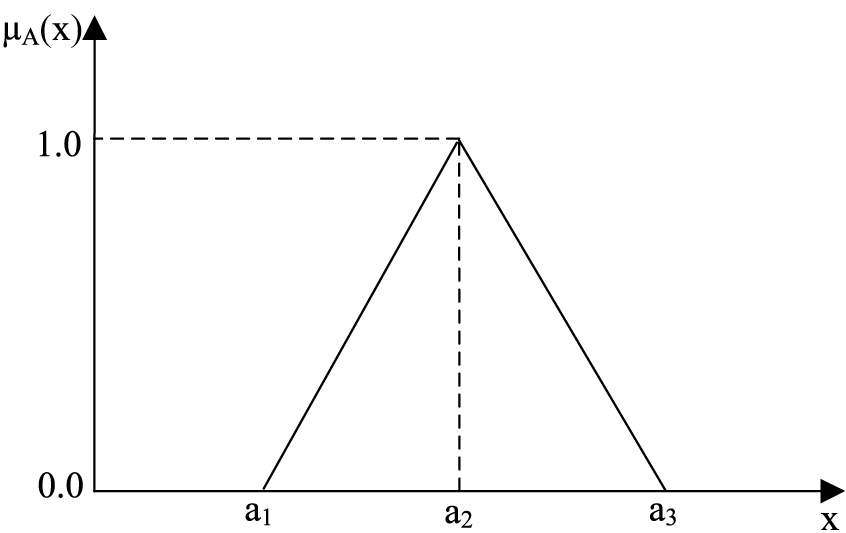
\includegraphics[width = 400px]{triangular_number.png}
\newline
\newline

$\mu_{A} \left( x \right)  =
\left\{
\begin{array}{lr}
0, & x < a_{1} \\
\\
x - a_{1} \over { a_{2}  - a_{1} } $ $, & a_{1} \leq x \leq a_{2} \\
\\
a_{3} - x \over{a_{3} - a_{2} } $ $, & a_{2} \leq x \leq a_{3} \\
\\
0, & x > a_{3}
\end{array}
\right.
$
\newline
\newline

\subsection{Аритметични операции - принцип на разширението}

Нека имаме две размити числа \~{A} $ = \varphi \left( a_{1} , b_{1} , c_{1} \right) $ и  \~{B} $ =  \varphi \left( a_{2} , b_{2} , c_{2} \right)$ .
\newline
Тогава:

\~{A} + \~{B} $ = \varphi \left( a_{1} + a_{2}, b_{1} + b_{2}, c_{1} + c_{2} \right)  $

\~{A} - \~{B} $ = \varphi \left( a_{1} - a_{2}, b_{1} - b_{2}, c_{1} - c_{2} \right)  $

\~{A} $ \cdot $ \~{B} $ = \varphi \left( min \left( a_{1} a_{2} , a_{1} c_{2} , c_{1} a_{2} , c_{1} c_{2} \right) , b_{1} b_{2} , max \left( a_{1} a_{2} , a_{1} c_{2} , c_{1} a_{2} , c_{1} c_{2} \right) \right)  $

\~{A} / \~{B} $ = \varphi \left( min \left( a_{1} / a_{2} , a_{1} / c_{2} , c_{1} / a_{2} , c_{1} / c_{2} \right) , b_{1} / b_{2} , max \left( a_{1} / a_{2} , a_{1} / c_{2} , c_{1} / a_{2} , c_{1} / c_{2} \right) \right)  $

\paragraph{}

Ето и алгоритъма реализиран чрез Python:

\begin{verbatim}

#!/usr/bin/python
import pylab



class FuzzyNumber:

  def __init__(self, left, peak, right):
    self.peak = peak
    self.left = left
    self.right = right
    self.all=[self.left, self.peak, self.right]

  def __add__(self, other):
    a = self.left + other.left
    b = self.peak + other.peak
    c = self.right + other.right
    return FuzzyNumber(a, b, c)

  def __sub__(self, other):
    a = self.left - other.left
    b = self.peak - other.peak
    c = self.peak - other.peak
    return FuzzyNumber(a, b, c)

  def __mul__(self, other):
    a = min(self.left * other.left, self.left * other.right, 
	    self.right * other.left, self.right * other.right)
    b = self.peak * other.peak
    c = max(self.left * other.left, self.left * other.right, 
	    self.right * other.left, self.right * other.right)
    return FuzzyNumber(a, b, c)

  def __div__(self, other):
    if (other.left != 0 and other.peak != 0 and other.right != 0):
      a = min(self.left / other.left, self.left / other.right, 
	      self.right / other.left, self.right / other.right)
      b = self.peak / other.peak
      c = max(self.left / other.left, self.left / other.right, 
	      self.right / other.left, self.right / other.right)
      return FuzzyNumber(a, b, c)

  def tuple(self):
     return tuple(self.all)

  def __str__(self):
    return 'FuzzyNumber(' + str(self.left) + ', ' + 
			  str(self.peak) + ', ' + str(self.right) + ')'

\end{verbatim}

На пример резултатът от събирането на размитите числа a = FuzzyNumber(1,3,9) и b = FuzzyNumber(4,6,8) е FuzzyNumber(5, 9, 17). Изчертава се следната графика: \newline
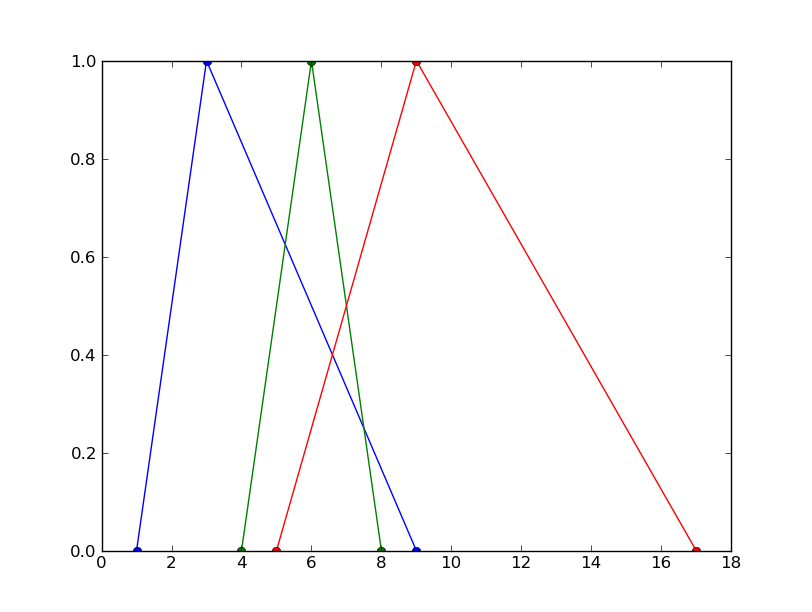
\includegraphics[width = 300px]{fuzzy_graphic.png}

В синьо и зелено са съответно числата $a$ и $b$, а в червено е резултатът от тяхното събиране.
Изчертаването на графиката е реализирано с помощта на библиотеката matplotlib по следния начин:

\begin{verbatim}

#plotting

def add_number(r, fig, ax):
  n = r.tuple()
  DATA = ((0, n[0]),
      (1, n[1]),
      (0, n[2]))

  (y,x) = zip(*DATA)

  ax.plot(x, y, marker='o')
  for i in xrange(len(DATA)):
    (x,y) = DATA[i]

if(__name__=='__main__'):
  fig = pylab.figure()
  ax = fig.add_subplot(111)
  for n in [a,b, a+b]: #, a-b, a*b, a/b]:
    add_number(n,fig,ax)
  print (a + b)
  pylab.show()

\end{verbatim}

\end{document}
